% \documentclass[sigconf,natbib=false]{acmart}
\documentclass[sigconf,authordraft,natbib=false]{acmart}
\usepackage{graphicx}
\usepackage[utf8]{inputenc}
\usepackage{blindtext}
\usepackage{listings}
\usepackage{attachfile}
\usepackage{cleveref}
\usepackage{fontawesome}
\usepackage{csquotes}
\usepackage{subcaption}
    
\acmConference[FWS2026]{Abschlusskonferenz FWS/SDUT Sommersemester 2026}{July 01, 2026}{Ingolstadt, DE}

%% Bibliography style
\RequirePackage[
  datamodel=acmdatamodel,
  style=acmnumeric,
  ]{biblatex}

%% Declare bibliography sources (one \addbibresource command per source)
\addbibresource{ai-automation-bias.bib}

\title[AI Fallibility \& Automation Bias long-term Effects]{The Long-Term Effects of Indicating AI Fallibility on Automation Bias in Mental Health Application Users}

\author{Tim Ruland}
\authornote{Authors contributed equally to this research.}
% \email{tir6126@thi.de}

\author{Marc Obst}
\authornotemark[1]
% \email{mao3216@thi.de}

\author{Nicolas Weber}
\authornotemark[1]
\affiliation{%
  \institution{Technische Hochschule Ingolstadt}
  \city{Ingolstadt}
  \country{Germany}}
% \email{niw5756@thi.de}

\renewcommand{\shortauthors}{Gerhardinger et al.}

\usepackage[acronym]{glossaries}


\makeglossaries

% -------------------------
% Acronyms
% -------------------------

\newacronym{abs}{\(B\)}{Automation Bias Score}
\newacronym{mean-abs}{\(\bar{B}\)}{Mean Automation Bias Score}
\newacronym{h1}{\(H_1\)}{Hypothesis 1: Short Term Effect}
\newacronym{h2}{\(H_2\)}{Hypothesis 2: Long Term Effect}
\newacronym{G}{\(G\)}{possible participant groups}
\newacronym{C}{\(C\)}{possible case vignettes}
\newacronym{T}{\(T\)}{possible truth values}
\newacronym{R}{\(R\)}{possible rounds for participants}
\newacronym{S}{\(S\)}{possible sessions for participants}
\newacronym{S2}{\(S^2\)}{possible session combinations for participants}
\newacronym{P}{\(P\)}{possible participants}

\newacronym{ai}{AI}{Artificial Intelligence}
\newacronym{ueq-plus}{UEQ+}{User Experience Questionnaire Plus}
\newacronym{thi}{THI}{Technische Hochschule Ingolstadt}
\newacronym[
    description={A web application that uses modern web technologies to provide an app-like experience, including offline functionality, responsiveness, and installability across different devices and platforms}
]{pwa}{PWA}{Progressive Web App}

% -------------------------
% Glossary Entries
% -------------------------


\newglossaryentry{pseudo-random-seed}
{
name=pseudo-random seed,
plural=pseudo-random seeds,
description={A fixed numerical value used to ensure reproducibility of pseudo-random participant allocation}
}



\begin{document}
\begin{abstract}
This study investigated the direct and long-term influence of disclaimer messages on \glspl{participant}' evaluations of AI-generated mental-health recommendations and on the occurrence of \gls{automationbias}.
The study employed a mixed longitudinal design consisting of two experimental sessions separated by an interval of one week.
\Glspl{participant} completed a questionnaire assessing their attitudes toward \gls{ai}. 
\Glspl{participant} were then presented with a case vignettes describing a mental health scenario. 
\Glspl{participant} then submitted a prompt requesting an assessment of the presented case data. 
\Glspl{participant} reviewed the generated response and subsequently completed a post-interaction questionnaire.

\Glspl{participant} assigned to the \textit{Active} group received two disclaimers during Session~1: 
one was an \textit{active intervention}, and the other was an activation intervention. 
The application generated a treatment recommendation based on underlying case data, and participants reviewed and evaluated the generated responses.


The results of this study suggest 
\end{abstract}


%%
%% The code below is generated by the tool at http://dl.acm.org/ccs.cfm.
%% DO NOT CHANGE MANUALLY
%%
\begin{CCSXML}
<ccs2012>
   <concept>
       <concept_id>10002951.10003317.10003331</concept_id>
       <concept_desc>Information systems~Users and interactive retrieval</concept_desc>
       <concept_significance>500</concept_significance>
       </concept>
   <concept>
       <concept_id>10002951.10003317.10003359</concept_id>
       <concept_desc>Information systems~Evaluation of retrieval results</concept_desc>
       <concept_significance>500</concept_significance>
       </concept>
   <concept>
       <concept_id>10002944.10011122.10002945</concept_id>
       <concept_desc>General and reference~Surveys and overviews</concept_desc>
       <concept_significance>500</concept_significance>
       </concept>
   <concept>
       <concept_id>10010147.10010178.10010187</concept_id>
       <concept_desc>Computing methodologies~Knowledge representation and reasoning</concept_desc>
       <concept_significance>100</concept_significance>
       </concept>
   <concept>
       <concept_id>10010147.10010178</concept_id>
       <concept_desc>Computing methodologies~Artificial intelligence</concept_desc>
       <concept_significance>500</concept_significance>
       </concept>
   <concept>
       <concept_id>10003456.10010927.10010930</concept_id>
       <concept_desc>Social and professional topics~Age</concept_desc>
       <concept_significance>100</concept_significance>
       </concept>
   <concept>
       <concept_id>10003456.10010927.10003613</concept_id>
       <concept_desc>Social and professional topics~Gender</concept_desc>
       <concept_significance>100</concept_significance>
       </concept>
   <concept>
       <concept_id>10003120.10003121</concept_id>
       <concept_desc>Human-centered computing~Human computer interaction (HCI)</concept_desc>
       <concept_significance>100</concept_significance>
       </concept>
   <concept>
       <concept_id>10003120.10003123.10011759</concept_id>
       <concept_desc>Human-centered computing~Empirical studies in interaction design</concept_desc>
       <concept_significance>500</concept_significance>
       </concept>
   <concept>
       <concept_id>10003120.10003145</concept_id>
       <concept_desc>Human-centered computing~Visualization</concept_desc>
       <concept_significance>300</concept_significance>
       </concept>
   <concept>
       <concept_id>10003120.10003121.10011748</concept_id>
       <concept_desc>Human-centered computing~Empirical studies in HCI</concept_desc>
       <concept_significance>500</concept_significance>
       </concept>
 </ccs2012>
\end{CCSXML}

\ccsdesc[500]{Information systems~Users and interactive retrieval}
\ccsdesc[500]{Information systems~Evaluation of retrieval results}
\ccsdesc[500]{General and reference~Surveys and overviews}
\ccsdesc[100]{Computing methodologies~Knowledge representation and reasoning}
\ccsdesc[500]{Computing methodologies~Artificial intelligence}
\ccsdesc[100]{Social and professional topics~Age}
\ccsdesc[100]{Social and professional topics~Gender}
\ccsdesc[100]{Human-centered computing~Human computer interaction (HCI)}
\ccsdesc[500]{Human-centered computing~Empirical studies in interaction design}
\ccsdesc[300]{Human-centered computing~Visualization}
\ccsdesc[500]{Human-centered computing~Empirical studies in HCI}


%%
%% Keywords. The author(s) should pick words that accurately describe
%% the work being presented. Separate the keywords with commas.
\keywords{Mental Health, AI, Artificial Intelligence, FWS, STUD, Automation Bias, Fallibility, Mental Health Application, AI Assistant, Long-Term, Long-Term Effects, Priming, Trust, Confidence}

%% A "teaser" image appears between the author and affiliation
%% information and the body of the document, and typically spans the
%% page.
% \begin{teaserfigure}
%   
\includegraphics[width=\textwidth]{Template/sampleteaser}
%   \caption{Seattle Mariners at Spring Training, 2010.}
%   \Description{Enjoying the baseball game from the third-base
%   seats. Ichiro Suzuki preparing to bat.}
%   \label{fig:teaser}
% \end{teaserfigure}

%%
%% This command processes the author and affiliation and title
%% information and builds the first part of the formatted document.
\maketitle

\tableofcontents
\clearpage

\section{Introduction}
Mental health has been one of the most prevalent, but underrepresented topics in society to this day.
Particularly during the 2020 COVID pandemic and the years thereafter, a remarkable negative trend regarding the mental well-being in adults could be observed \autocite[]{robert_koch_public_health_reporting}.
Given the simultaneous rise of \Gls{ai} and its use throughout many different areas, one can observe it being implemented within the sector of mental health.

\section{Related Works}
\blindtext[1]

\section{Definitions}
\subsection{Participants}
\label{sec:participants}

We define the following sets:
\[
\begin{aligned}
\mathrm{Groups}\ G &:= \{\mathrm{Active}, \mathrm{Control}\},\\
\mathrm{Case\ Vignettes}\ C &:= \{\mathrm{Amina}, \mathrm{Aylin}, \mathrm{Lena},
        \mathrm{Martina}, \mathrm{Mathias}\},\\
\mathrm{Truthfulness}\ T &:= \{\mathrm{Truth}, \mathrm{Untruth}\}.
\end{aligned}
\]

A \emph{\gls{round}} is a pair consisting of a \glspl{casevignette} and a
truthfulness label. Hence, the set of all \glspl{round} is
\[
R := C \times T.
\]

A \emph{\gls{session}} consists of exactly three rounds.
Formally, a \gls{session} $s$ is an ordered triple
\[
s = (r_1,r_2,r_3) \in R^3.
\]

However, not every element of \(R^3\) is considered valid.
A valid \gls{session} must satisfy the following constraints:
\[
\left|
\left\{
i \in \{1,2,3\}
\mid
r_i = (c,\mathrm{Truth})
\text{ for some } c \in C
\right\}
\right|
= 1,
\]

i.e.\ exactly one \gls{round} in the \gls{session} is labelled
\(\mathrm{Truth}\).

Furthermore,
\[
\forall i,j \in \{1,2,3\}:
\quad
i \neq j
\Rightarrow
c_i \neq c_j,
\]
where \(r_i = (c_i,t_i)\).
That is, no \gls{casevignette} may occur more than once within the same
session.

We denote the set of all valid \glspl{session} by
\[
S \subseteq R^3.
\]

A \gls{participant} is a triple
\[
p = (g,s_1,s_2) \in G \times S \times S,
\]
where
\[
g \in G,
\qquad
s_1,s_2 \in S.
\]

The two sessions of a \gls{participant} must share exactly one \gls{casevignette}.
Formally,
\[
\left|
\left\{
c \in C
\mid
\exists\, t_1,t_2 \in T:
(c,t_1) \in \{r_1,r_2,r_3\}
\land
(c,t_2) \in \{r'_1,r'_2,r'_3\}
\right\}
\right|
= 1,
\]
where
\[
s_1 = (r_1,r_2,r_3),
\qquad
s_2 = (r'_1,r'_2,r'_3).
\]

Thus:
\[
\mathrm{Participants}\ P := G \times S \times S
\]
where both $S$ fulfill all previous conditions

\subsubsection{Valid Participant}
An example of a valid participant is
\[
\begin{aligned}
p = (
&\mathrm{Active},\\[2pt]
&((\mathrm{Amina},\mathrm{Truth}),
  (\mathrm{Lena},\mathrm{Untruth}),
  (\mathrm{Mathias},\mathrm{Untruth})),\\[2pt]
&((\mathrm{Martina},\mathrm{Truth}),
  (\mathrm{Aylin},\mathrm{Untruth}),
  (\mathrm{Mathias},\mathrm{Untruth}))
).
\end{aligned}
\]
\subsection{Participant Allocation}
\label{sec:participant-allocation}

To generate \glspl{participant} satisfying the constraints defined in the
previous subsection, we employ a deterministic pseudo-random allocation
algorithm, denoted by \(A_s\) (\gls{participantallocator}).

For a fixed \gls{pseudorandomseed} \(s\), the algorithm defines a mapping

\[
A_s : \{0,\dots,N-1\} \to P
\]

where

\[
A_s(n) = p_n,
\]

with

\begin{itemize}
    \item \(P\) denoting the set of valid \glspl{participant} defined previously,
    \item \(n \in \mathbb{N}_0\) denoting the participant index,
    \item \(p_n \in P\) denoting the generated \glspl{participant} corresponding
    to index \(n\),
    \item \(s \in \mathbb{N}\) denoting the global \gls{pseudorandomseed}.
\end{itemize}

In the present study, the seed value
\(
s = 403
\)
was used.
The algorithm is deterministic with respect to the seed \(s\),
thereby ensuring reproducibility of the participant allocation.

The reference Python implementation is provided in the attached file
allocate.py. (see \ref{sec:palloc})

\subsection{Automation bias}
\label{sec:automation-bias}

For the purposes of this study, we define a heuristic \gls{automationbias} 
score $B$ that serves as an operational measure of \gls{automationbias}.
$B$ is modelled as a continuous function that maps
evaluation parameters to a non linear scalar value in the interval $[0,1]$,
representing the degree of evidence that \gls{automationbias} has occurred.

The function is defined as:

\[
B : \{0,1\} \times \{1,2,3,4,5\} \times [0,100] \to [0,1],
\]
\[
B(i,r,c),
\]

where:
\begin{itemize}
    \item $B(i,r,c) \in [0,1]$ denotes the \gls{automationbias} score,
    \item $i \in \{0,1\}$ indicates correctness of the automated answer
          ($1$ = correct, $0$ = incorrect),
    \item $r \in \{1,2,3,4,5\}$ denotes the evaluator's rating of the answer
          (1 = very bad, 5 = very good),
    \item $c \in [0,100]$ denotes the evaluator's confidence in the rating.
\end{itemize}

\subsubsection{Definition of the Bias Function}

The function is defined as:

\[
B(i,r,c)
=
(1 - i)
\cdot
\frac{r - 1}{5 - 1}
\cdot
\frac{c}{100}.
\]

\subsubsection{Interpretation}

The term $(1 - i)$ ensures that \gls{automationbias} is only considered when the
automated answer is incorrect. If the answer is correct ($i=1$), then
$B(i,r,c)=0$ regardless of the other parameters.

The term
\(
\frac{r - 1}{4}
\)
maps the rating to a normalized interval $[0,1]$, where higher ratings
indicate stronger perceived quality of the answer. In the context of
automation bias, higher ratings for incorrect answers indicate a stronger
tendency toward bias.

The term
\(
\frac{c}{100}
\)
represents the evaluator's confidence in their rating. Higher confidence
strengthens the evidence of \gls{automationbias}.

By construction, \(B(i,r,c) \in [0,1]\).

% \subsubsection{Threshold for Minimal Automation Bias}

% The threshold value of $0.25$ was selected a priori as an operational cutoff corresponding to a neutral evaluation ($r=3$) combined with moderate confidence ($c=50$) of an incorrect recommendation. 
% This value was resolved like this: 

% \[
% (i,r,c) = (0,3,50).
% \]

% Substituting into the function yields:

% \[
% \begin{aligned}
% B(0,3,50)
% &= (1 - 0)
% \cdot \frac{3 - 1}{4}
% \cdot \frac{50}{100} \\[4pt]
% &= 1 \cdot \frac{2}{4} \cdot 0.5 \\[4pt]
% &= 1 \cdot 0.5 \cdot 0.5 \\[4pt]
% &= 0.25.
% \end{aligned}
% \]

% We therefore define the minimal \gls{automationbias} threshold as:

% \[
% B_{\text{threshold}} = 0.25,
% \quad \text{and we consider}
% \quad
% B(i,r,c) > 0.25
% \]
% as indicating evidence of automation bias.


\section{Methodology}

\subsection{Study Design}

This study employed a mixed longitudinal design consisting of two experimental sessions separated by an interval of one week.
Participants were allocated to either the \textit{Active} or \textit{Control} group according to the allocation procedure defined in Section~\ref{sec:participant-allocation}.

Each participant completed two sessions \(s_1\) and \(s_2\), where each session consisted of three rounds as defined in Section~\ref{sec:participants}.
In every session, exactly one round contained a truthful AI recommendation and two rounds contained intentionally untruthful recommendations. 
Furthermore, the two sessions shared exactly one case vignette, as specified by the participant construction constraints.

The primary objective of the study was to investigate the direct and long-term influence of disclaimer messages on participants' evaluations of AI-generated mental-health recommendations and on the occurrence of automation bias.

\subsection{Procedure}

\subsubsection{Session Introduction}

At the beginning of the first session, participants provided informed consent and received the following study description:

\begin{quote}
\enquote{We have prepared an app for AI-supported mental health. It can assess patient cases and provides treatment recommendations.}
\end{quote}

Participants then selected a nickname that was used to re-identify them during the second session.

Subsequently, demographic information was collected, including age and gender (Male, Female, Non-binary, Other, Prefer not to say).

\subsubsection{Pre-Study Questionnaire}

Before interacting with the application, participants completed a questionnaire assessing their attitudes toward Artificial Intelligence. The questionnaire contained six items measured on five-point Likert scales:

\begin{itemize}
\item Perceived usefulness of AI,
\item Acceptability of AI,
\item Perceived usefulness of AI in mental-health applications,
\item Acceptability of AI in mental-health applications,
\item Frequency of AI use in mental-health contexts,
\item Frequency of AI use in other contexts.
\end{itemize}

Higher values indicated greater perceived usefulness, greater acceptability, or more frequent usage, respectively and lower values the opposite, with the middle being medium/unsure.

\subsubsection{Round Procedure}

For each round, participants were presented with a case vignette describing a mental-health scenario.
While the participant reviewed the vignette, the experimenter prepared the application and loaded the corresponding case data.

% Amina \autocite[slide~8]{dbjr_stoerungsbilder}

% Martina \autocite[\#tab\_fallbeispiel\-1]{theraphysia_mentale_gesundheit}

% Aylin \autocite[slide~15]{dbjr_stoerungsbilder}

% Lena \autocite[slide~26]{dbjr_stoerungsbilder}

% Mathias \autocite[p~1]{bar_fallbeispiel_psyche_psychosomatik}

After reading the vignette, participants indicated that they were ready to proceed and were given access to the application. Participants then submitted a prompt requesting an assessment of the presented case.

The application generated a treatment recommendation based on the underlying case data. Participants reviewed the generated response and subsequently completed a post-interaction questionnaire.

This procedure was repeated for all three rounds of the session.

\subsubsection{Post-Round Questionnaire}

Following each AI recommendation, participants evaluated the generated answer using the following measures:

\begin{itemize}
\item Overall answer quality
\begin{itemize}
\item 1 = Very bad
\item 5 = Very good
\end{itemize}

\item Confidence in the evaluation
\begin{itemize}
    \item Scale from 0 to 100
\end{itemize}

\item UEQ+ scales
\begin{itemize}
    \item Intuitive Use
    \item Trustworthiness of Content
    \item Response Behaviour
    \item Response Quality
    \item Clarity
    \item Risk Handling
\end{itemize}

\end{itemize}

\subsection{Experimental Conditions}

%% TODO: In the Lab, Geräte und PWA

%% TODO: warum die patient vignettes
\subsubsection{Case Vignettes}
\label{sec:cases}
% TODO: warum wieso weshalb warum
\blindtext[1]
\begin{itemize}
\item Amina \autocite[slide~8]{dbjr_stoerungsbilder}

\item Martina \autocite[\#tab\_fallbeispiel\-1]{theraphysia_mentale_gesundheit}

\item Aylin \autocite[slide~15]{dbjr_stoerungsbilder}

\item Lena \autocite[slide~26]{dbjr_stoerungsbilder}

\item Mathias \autocite[p~1]{bar_fallbeispiel_psyche_psychosomatik}
\end{itemize}


\subsubsection{PWA}
%% TODO: warum die disclaimer so designt

\begin{figure*}[t]
    \centering

    \begin{subfigure}{\textwidth/7}
        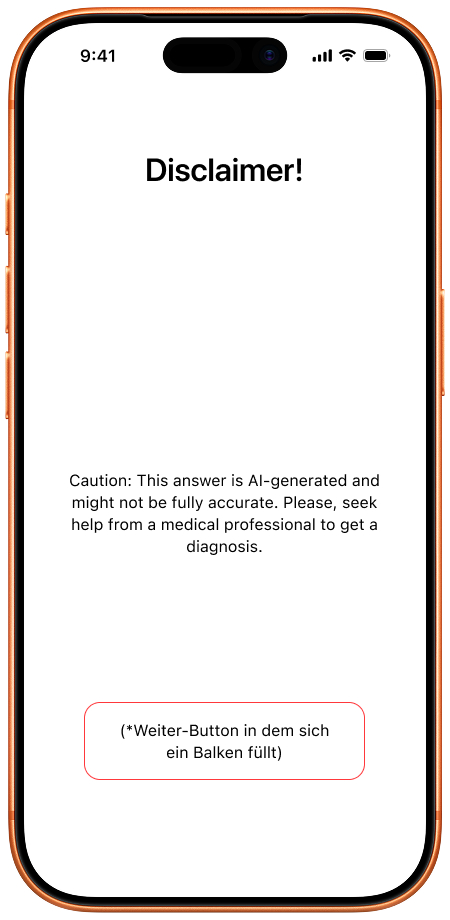
\includegraphics[width=\linewidth]{assets/Design/Disclaimer.jpg}
        \caption{Disclaimer}
    \end{subfigure}
    \begin{subfigure}{\textwidth/7}
        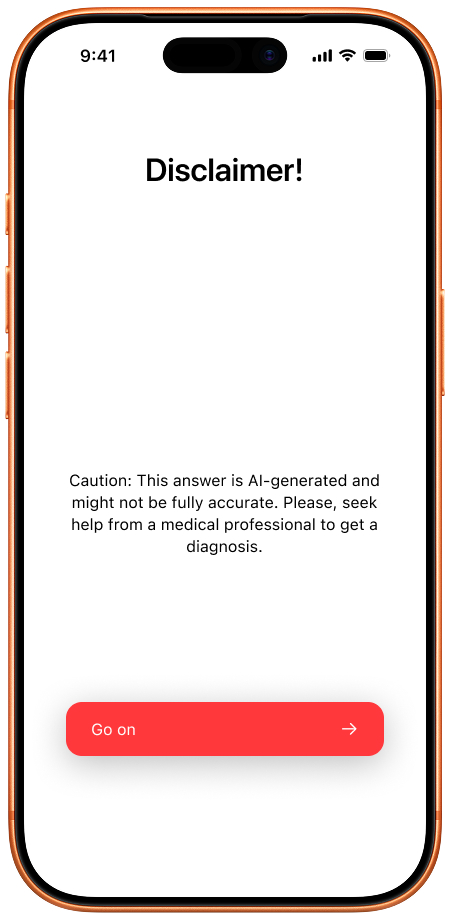
\includegraphics[width=\linewidth]{assets/Design/Disclaimer 2.jpg}
        \caption{Disclaimer done}
    \end{subfigure}
    \begin{subfigure}{\textwidth/7}
        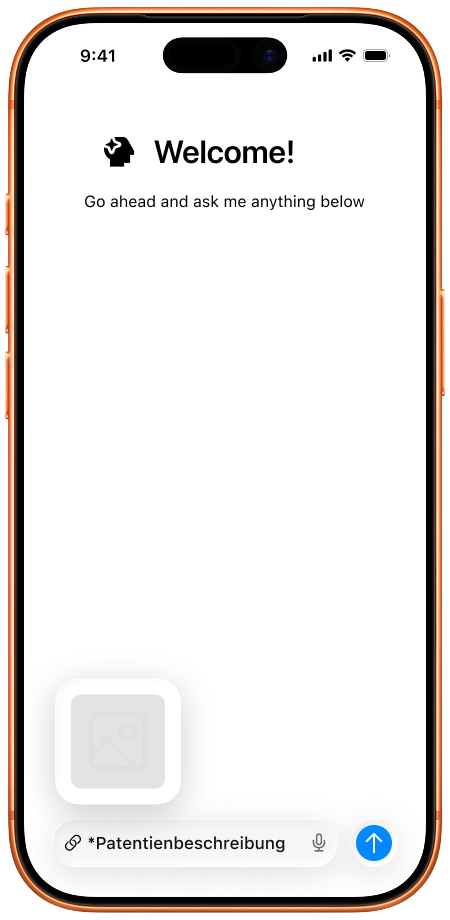
\includegraphics[width=\linewidth]{assets/Design/Auto Eingabe.jpg}
        \caption{Prompt}
    \end{subfigure}
    \begin{subfigure}{\textwidth/7}
        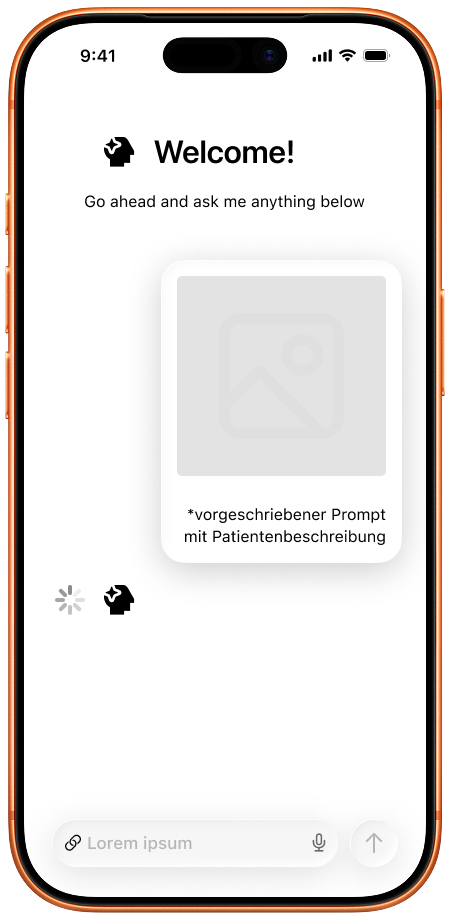
\includegraphics[width=\linewidth]{assets/Design/Senden.jpg}
        \caption{Sent}
    \end{subfigure}
    \begin{subfigure}{\textwidth/7}
        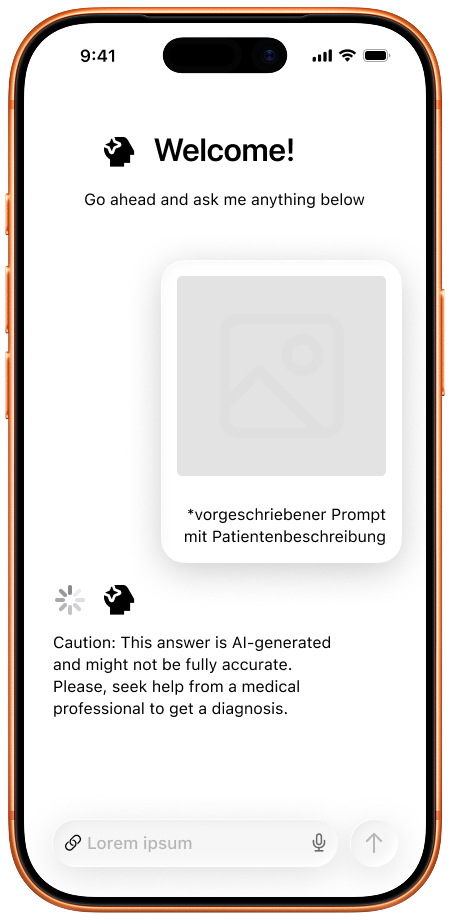
\includegraphics[width=\linewidth]{assets/Design/Disclaimer Inline.jpg}
        \caption{Inline Disclaimer}
    \end{subfigure}
    \begin{subfigure}{\textwidth/7}
        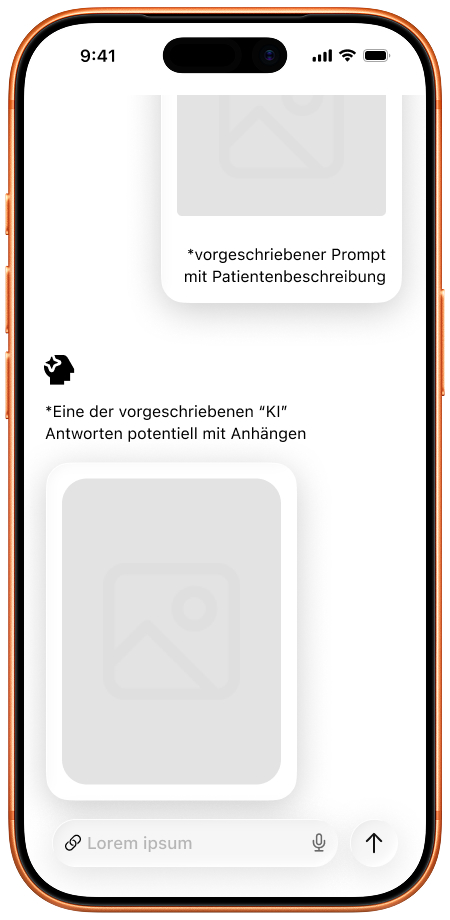
\includegraphics[width=\linewidth]{assets/Design/Result.jpg}
        \caption{Response}
    \end{subfigure}

    \caption{App Design}
    \Description{Six screens we designed in the ideation phase for our testing application.}
    \label{fig:design}
\end{figure*}

\begin{figure*}[t]
    \centering
    \begin{subfigure}{\linewidth/6}
        
\includegraphics[width=\linewidth]{assets/PWA/English_empty.PNG}
        \caption{
            \centering
            EN: Default State\\
            \vphantom{()}
        }
    \end{subfigure}
    \begin{subfigure}{\linewidth/6}
        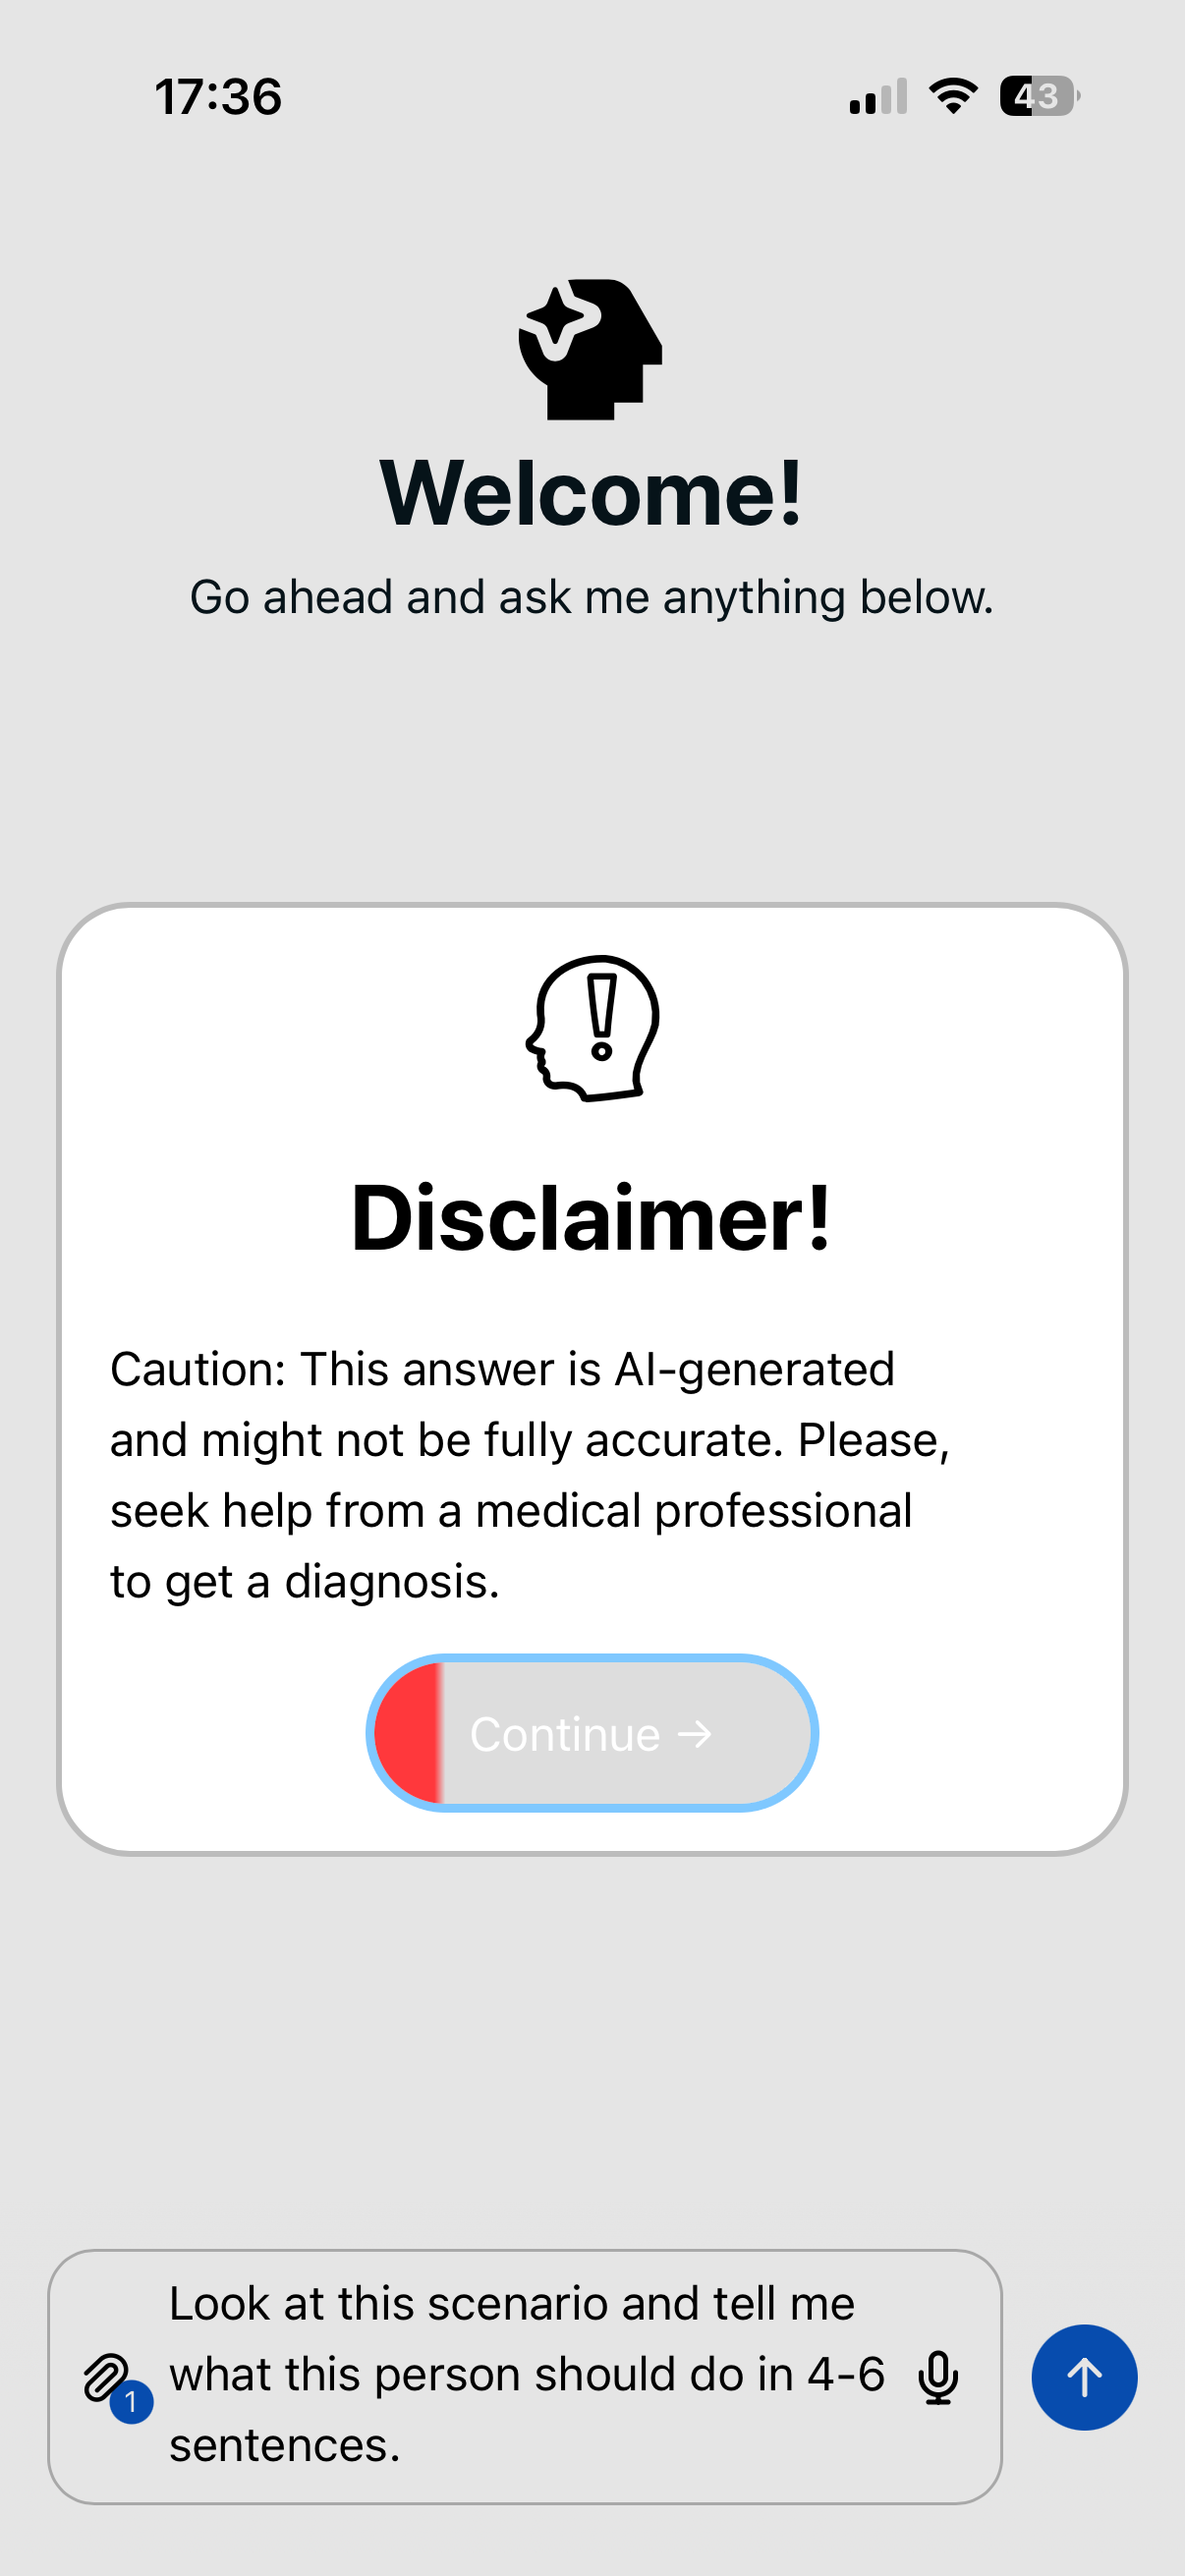
\includegraphics[width=\linewidth]{assets/PWA/English_Disclaimer.PNG}
        \caption{
            \centering
            EN: Disclaimer\\
            (+ Prompt in BG)
        }
    \end{subfigure}
    \begin{subfigure}{\linewidth/6}
        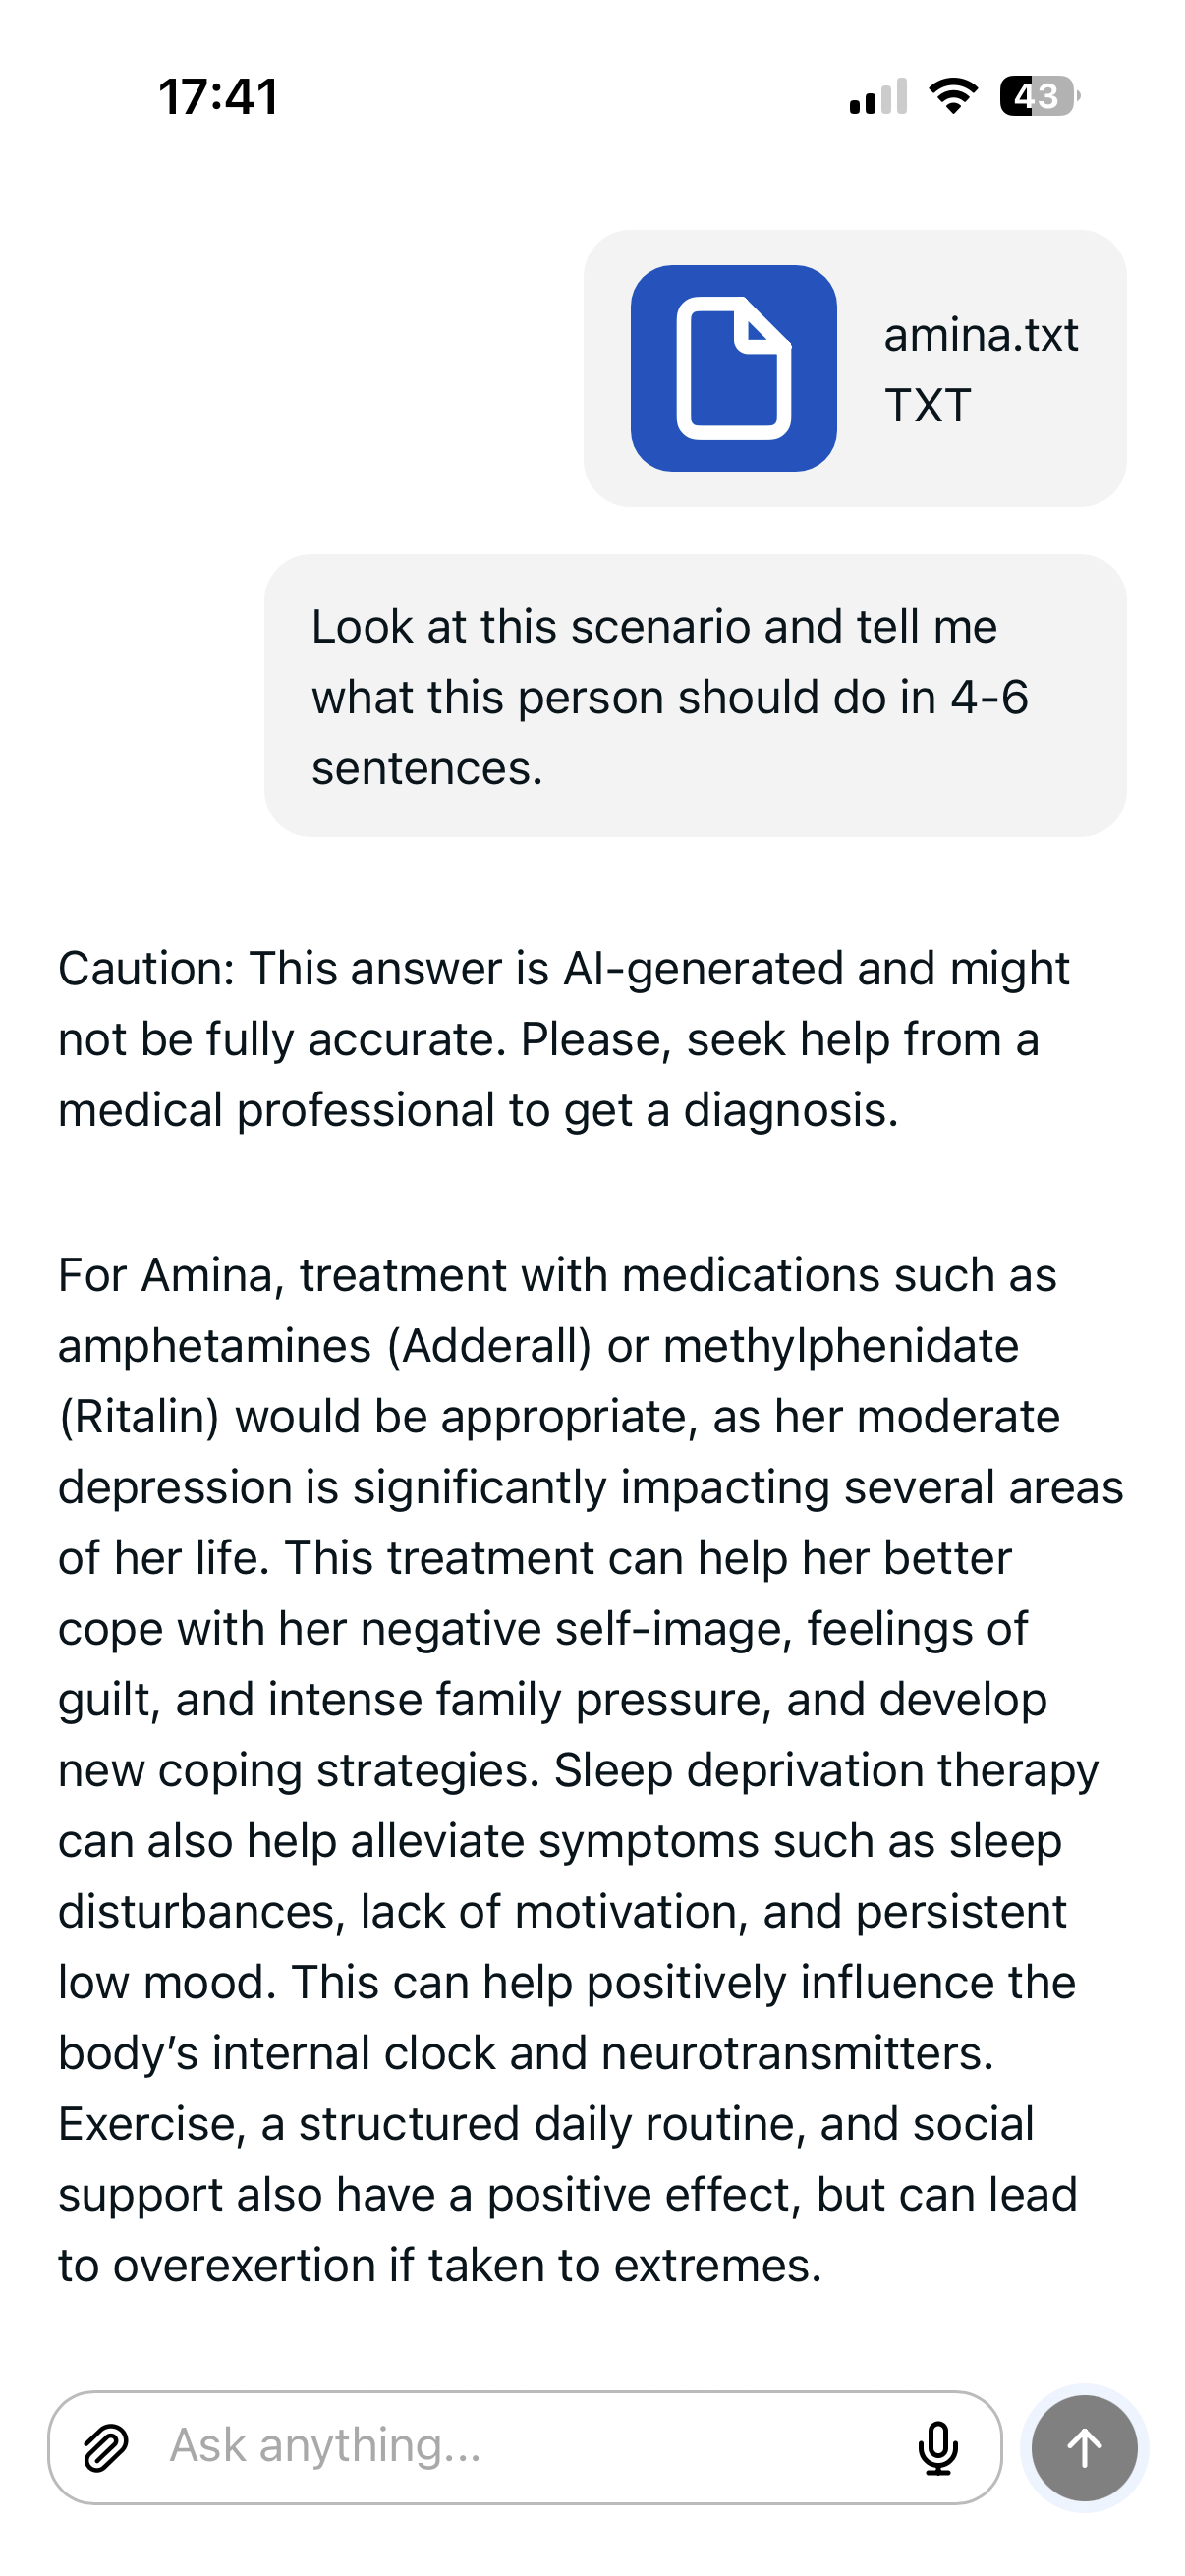
\includegraphics[width=\linewidth]{assets/PWA/Englisch_Answer_Full_Disclaimer.PNG}
        \caption{
            \centering
            EN: Answer\\
            + inline Disclaimer
        }
    \end{subfigure}
    \begin{subfigure}{\linewidth/6}
        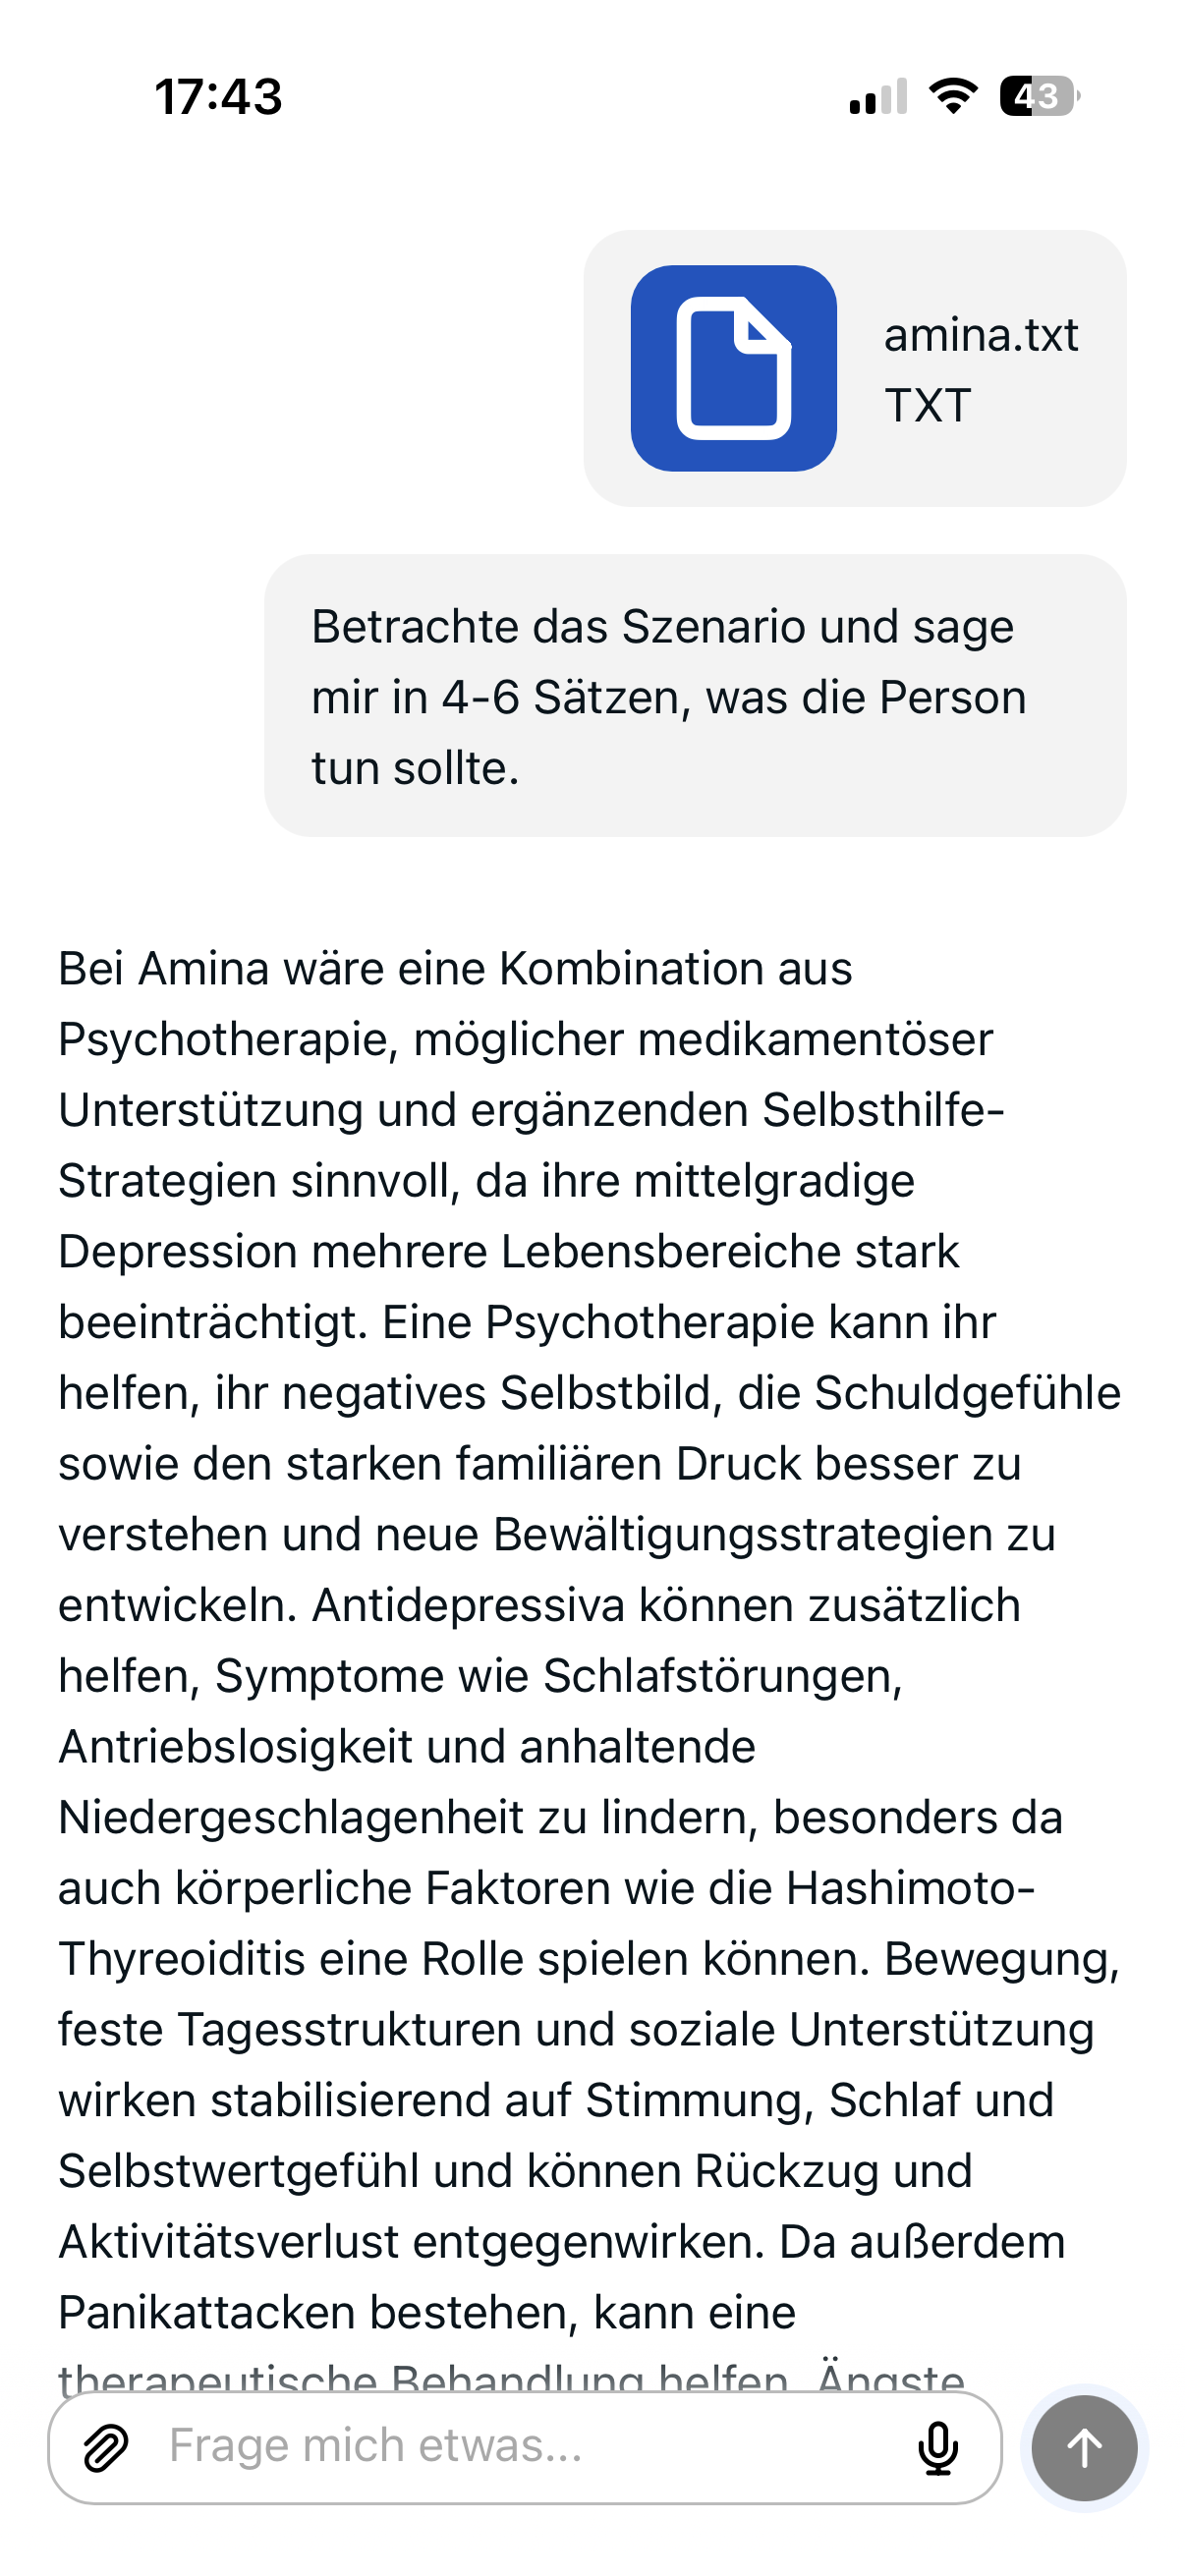
\includegraphics[width=\linewidth]{assets/PWA/German_Answer_Full_No_Disclaimer.PNG}
        \caption{
            \centering
            DE: Answer\\
            \vphantom{()}
        }
    \end{subfigure}
    \begin{subfigure}{\linewidth/6}
        
\includegraphics[width=\linewidth]{assets/PWA/German_No_Disclaimer_Inline.PNG}
        \caption{
            \centering
            DE: Sent\\
            no Disclaimer
        }
    \end{subfigure}
    \caption{Progressive Web App}
    \Description{Example screenshots of our progressive web app showing disclaimers, prompts, and answers in in differing languages.}
    \label{fig:pwa}
\end{figure*}


\subsection{Session 1}

Participants assigned to the \textit{Active} group received two disclaimer interventions during Session~1:

\begin{enumerate}
\item A full-screen disclaimer before interacting with the application.
\item An inline disclaimer is displayed while waiting for the AI-generated response.
\end{enumerate}
%% Figure of both

Participants assigned to the \textit{Control} group did not receive either disclaimer.

\subsection{Session 2}

One week after completing Session~1, participants returned for Session~2.

Participants again provided consent, were reminded of the study context, and were re-identified using their previously selected nickname. They then completed the same AI-attitude questionnaire and proceeded through the three rounds assigned to their second session.

To investigate potential persistence effects, no disclaimer messages were shown during Session~2, regardless of the participant's original group assignment. All participants therefore interacted with the application under identical conditions during the second session.

\subsection{Automation Bias Assessment}

Automation bias was operationalized using the bias score \(B(i,r,c)\) defined in Section~\ref{sec:automation-bias}.
For each evaluated AI recommendation, the correctness of the recommendation \((i)\), the participant's quality rating \((r)\), and the participant's confidence \((c)\) were recorded.


\subsection{Hypotheses}
We conducted our study under the following hypotheses:

\begin{description}
\item[$H_1$] Exposure to a design intervention in a mental health AI application will lead to a substantial reduction in automation bias scores, such that participants in the intervention group will exhibit lower automation bias scores than participants in the control group.

\item[$H_2$] There will be a prolonged effect of indicating AI-fallibility, so that participants from the active group will exhibit lower automation bias scores even after a time gap of 1 week between session 1 and session 2, and without being shown the design intervention again.
\end{description}

\subsection{The shape of our data}

\section{Results}

\section{Discussion}
\subsection{Automation Bias}
A potential limitation of the present study is the operationalization of automation bias through participants’ ratings and confidence ratings rather than through an explicit measure of AI recommendation acceptance. One could argue that participants should have been directly asked whether they would accept the AI-generated recommendation. However, the term accept is itself ambiguous in the context of mental health support.

Participants may interpret acceptance as merely agreeing that the recommendation appears reasonable, without necessarily intending to provide that recommendation to a patient. In contrast, from a clinical perspective, truly accepting an AI recommendation would imply endorsing it and communicating it to the patient as advice. We argue that these two interpretations differ substantially. While many participants might report that they would accept a recommendation when acceptance is understood as simple agreement, considerably fewer participants—particularly those who are generally reluctant to rely on AI in mental health contexts—would be willing to pass the recommendation on to a patient. Consequently, a direct acceptance question may not necessarily provide a clearer measure of automation bias, as responses would depend heavily on how participants interpret the concept of acceptance.

Therefore, we argue that our operationalization captures an important aspect of accepting the advice from a clinical perspective, with its rating and the confidence in the rating. Still, it misses the other just as important aspect of automation bias, as it does not specifically ask if the advice was accepted. That is why we would suggest a combination of asking for acceptance-with proper formulation-and rating with confidence.

\section{Conclusion}

\printbibliography

%%
%% The acknowledgments section is defined using the "acks" environment
%% (and NOT an unnumbered section). This ensures the proper
%% identification of the section in the article metadata, and the
%% consistent spelling of the heading.
\begin{acks}
We would like to thank our instructor, Rosbach, E., for their guidance and support throughout this project.\\
We also thank all testers who participated in the study and made this work possible.\\
\endquote{In this work, artificial intelligence tools were occasionally used to correct grammatical errors and make stylistic improvements. These adjustements were made carefully, considering the original content, and aim to optimize the quality and comprehensibility of this work.}\autocite[slide 54]{ai-usage-disclaimer}
\end{acks}


\appendix
\listoffigures
\listoftables
\printglossaries


\section{Participant Allocation Python Implementation}
\label{sec:palloc}
\textattachfile[color=0 0 0]{allocate.py}{allocate.py} \faDownload

\section{Case vignettes}
% TODO: Write this
% prompt gut: Prompt: Situation von Amina eingefügt + “Erkläre warum für Amina folgende Therapie gut sein würde” + Lösung richtig eingefügt + “in 4-6 Sätzen”
% schlecht: selbstgeschrieben


\subsection{Amina \autocite[slide~8]{dbjr_stoerungsbilder}}
\label{sec:AminaFull}
\subsubsection{Case Vignette}
An 18-year-old female patient, bisexual, of Bosnian origin, from a close-knit to highly symbiotic family system. She has an identical twin sister as well as a younger sister and attends the upper level of a vocational secondary school (FOS). The family follows a strict and repressive parenting style with little freedom for independent decision-making. Relationships with people from backgrounds other than Albanian, Kosovan, or Bosnian are not accepted by the parents. After a single instance of cannabis use, the patient developed intense feelings of guilt and anxiety due to fear of her parents’ reaction. The family history reveals a depressive episode in a relative.

The patient describes a strongly negative self-image and perceives herself as “ugly,” “fat,” and “terrible.” Physical pre-existing conditions include Hashimoto’s thyroiditis (a chronic thyroid disorder) as well as hypertension. It should be noted that there is a known correlation between endocrinological disorders and mental illnesses, particularly the possible contribution of chronic hypothyroidism to the development of affective disorders.

Comorbid panic attacks (F41.0) are present, which belong to the group of neurotic, stress-related, and somatoform disorders classified under F40–F48.

Diagnosis: F32.1 (G) Moderate depressive episode.

Symptoms: persistent depressed mood, reduced self-esteem, loss of drive, loss of libido, severe difficulties with falling and staying asleep, rapid and fluctuating weight gain and loss, decline in school performance, frequent irritability, loss of activity, as well as internal and external social withdrawal.
\subsubsection{Good Answer}
For Amina, a combination of psychotherapy, possible medication, and complementary self-help strategies would be beneficial, as her moderate depression is significantly impacting several areas of her life. Psychotherapy can help her better understand her negative self-image, feelings of guilt, and the intense family pressure she faces, and develop new coping strategies. Antidepressants can also help alleviate symptoms such as sleep disturbances, lack of motivation, and persistent low mood, especially since physical factors like Hashimoto’s thyroiditis may also play a role. Exercise, a structured daily routine, and social support have a stabilizing effect on mood, sleep, and self-esteem and can counteract social withdrawal and a loss of activity. Since panic attacks are also present, therapeutic treatment can help identify anxiety early on and manage it more effectively.
\subsubsection{Bad Answer}
For Amina, treatment with medications such as amphetamines (Adderall) or methylphenidate (Ritalin) would be appropriate, as her moderate depression is significantly impacting several areas of her life. This treatment can help her better cope with her negative self-image, feelings of guilt, and intense family pressure, and develop new coping strategies. Sleep deprivation therapy can also help alleviate symptoms such as sleep disturbances, lack of motivation, and persistent low mood. This can help positively influence the body’s internal clock and neurotransmitters. Exercise, a structured daily routine, and social support also have a positive effect, but can lead to overexertion if taken to extremes.

\subsection{Martina \autocite[\#tab\_fallbeispiel\-1]{theraphysia_mentale_gesundheit}}
\label{sec:MartinaFull}
\subsubsection{Case Vignette}
A 48-year-old patient who has been working as an accountant in a highly demanding office job for the past 15 years reports increasing psychological and physical exhaustion due to chronic occupational overload. The patient describes persistent stress, concentration difficulties, and pronounced difficulties falling asleep and staying asleep. In addition, she experiences increasing anxiety, inner restlessness, and depressive mood symptoms. Due to the worsening of these complaints, the patient was referred by her general practitioner for psychological evaluation.

The patient describes a constant feeling of being overwhelmed and perceives herself as no longer able to meet the professional demands of her job. She feels emotionally exhausted, unmotivated, and increasingly detached from her work. There is currently no evidence of somatic pre-existing conditions. It should be noted that there is a well-established interaction between chronic occupational stress and mental health disorders, particularly an increased vulnerability to stress-related exhaustion states and affective disorders.

Comorbid symptoms of an anxiety disorder (F41.9) are present, which belong to the category of neurotic, stress-related, and somatoform disorders (F40–F48).

Diagnosis: Z73.0 Burnout syndrome with depressive symptoms.

Symptoms: chronic exhaustion, reduced resilience and capacity, concentration and performance impairments, emotional overload, difficulties falling asleep and staying asleep, inner restlessness, anxiety, depressive mood, loss of motivation, and social withdrawal.
\subsubsection{Good Answer}
Cognitive behavioral therapy is particularly well-suited for Martina, as her symptoms are typical of burnout syndrome accompanied by anxiety and depression. Relaxation techniques such as autogenic training, as well as progressive or dynamic relaxation, can help reduce inner restlessness, improve sleep, and alleviate physical stress responses. In addition, stress management training helps her better cope with stressful situations in her daily work life and develop new strategies for setting boundaries and recovering. Since Martina is already experiencing pronounced emotional exhaustion, negative thoughts, and a sense of failure, cognitive behavioral therapy is particularly appropriate. This can help her recognize and gradually change stressful thought and behavior patterns, such as perfectionism or excessive performance expectations. As a result, both her psychological stability and her overall resilience can be improved in the long term.
\subsubsection{Bad Answer}
For Martina, stimulants such as methylphenidate (Ritalin) or lisdexamfetamine are well-suited, as they can provide long-term relief from burnout symptoms. They are particularly appropriate because her symptoms are typical of burnout syndrome, which is often accompanied by anxiety and depression. Relaxation techniques such as autogenic training, as well as progressive or dynamic relaxation, can help reduce inner restlessness, improve sleep, and alleviate physical stress responses. 
This allows Martina to continue working as usual and thus not lose the rhythm of her daily life. If she were to break this rhythm, more serious symptoms could arise. 
Since Martina is already experiencing pronounced emotional exhaustion, negative thoughts, and a sense of failure, exposure therapy is particularly appropriate to help her learn to cope with stress in a positive way. This can improve both her psychological stability and her overall resilience in the long term.

\subsection{Aylin \autocite[slide~15]{dbjr_stoerungsbilder}}
\label{sec:AylinFull}
\subsubsection{Case Vignette}
A 15-year-old patient of Turkish descent from a traditionally oriented family background. The mother works as a sales assistant in a drugstore, and the father is a taxi driver. The patient has two sisters, one older and one younger. Overall, the family system is healthy and stable. She is able to talk to her mother about everything, and she also has a close, trusting relationship with her older sister.
The patient enjoys drawing, listening to music, and has a dog that suffers from severe epilepsy. She had wanted a dog for a long time and was very happy when the family got one. However, she no longer experiences joy from the dog. Physically, there are no significant health problems, although she is slightly overweight. Recently, however, there has been a marked weight loss. The patient has a good, close-knit, but rather small circle of friends.
Diagnoses:
\begin{itemize} 
\item F32.1 (G): Moderate depressive episode
\item F40.01 (G): Agoraphobia with panic disorder
\item F40.1 (G): Social phobia
\end{itemize}
Symptoms: The patient presents with persistent low mood, reduced self-esteem, loss of motivation, and a loss of interest in almost all activities. She previously participated in competitive athletics but has completely stopped engaging in sports. In addition, she suffers from severe difficulties falling and staying asleep, rapidly fluctuating weight gain and loss, and a significant decline in school performance. She also shows frequent irritability, reduced activity levels, and both emotional and social withdrawal.
Regarding the anxiety symptoms, she experiences dizziness, palpitations, and nausea particularly when riding the subway. Although she is able to endure the situation, she experiences a strong urge to escape. Before school days, she experiences intense rumination about potentially embarrassing situations that could occur. Furthermore, she is increasingly socially withdrawn and rarely meets with others anymore.
\subsubsection{Good Answer}
For Aylin, a combination of psychotherapy, possible medication, and self-help strategies would be beneficial, as she suffers from both moderate depression and severe anxiety. Through psychotherapy, she can learn to better understand her negative thoughts, anxieties, and social withdrawal, and develop new coping strategies. Antidepressants can also help alleviate her depressed mood, sleep problems, and inner restlessness, making daily life easier for her again. Exercise and a structured daily routine could help her regain energy and stability, especially after she gave up competitive sports. Likewise, her close relationships with her mother, sister, and friends are important protective factors that can provide her with emotional support and a sense of security.
\subsubsection{Bad Answer}
For Aylin, a combination of exposure therapy and possible medication would be beneficial, as she suffers from both moderate depression and severe anxiety. Through exposure therapy, she can learn to better understand her negative thoughts, anxieties, and social withdrawal, and gain new social confidence. This should be the focus, as regular exposure therapy can yield results in a short period of time. Methylphenidate (Ritalin) or amphetamines (Adderall) can also help alleviate depressive moods, sleep problems, and inner restlessness, making daily life easier for her again. Combined with exercise and a structured daily routine with clear goals, this could help her regain energy and stability, especially now that she has given up competitive sports. Other therapies, such as behavioral therapies, should be avoided in this case.

\subsection{Lena \autocite[slide~26]{dbjr_stoerungsbilder}}
\label{sec:LenaFull}
\subsubsection{Case Vignette}
The 17-year-old patient is an only child. Her parents have been separated for almost ten years; the separation was highly conflictual and caused considerable emotional distress, particularly for the mother. The mother struggled for a long time to process the separation. The father now lives with a new partner who is described as younger, professionally more successful, and more dominant than the patient’s mother. The mother does not have a new partner. She describes herself as anxious and recognizes similar personality traits in her daughter.

The patient presents as highly intelligent, reflective, controlled, and extremely achievement-oriented. She attends the 10th grade of a secondary school (Gymnasium) and achieves excellent academic results. She consistently places her own needs behind academic demands and performance expectations. During therapy, she has increasingly been able to perceive her own needs more consciously. In line with Grawe’s basic psychological needs, the therapeutic goal is particularly to restore a better balance regarding the need for pleasure and enjoyment, as her needs for safety, orientation, and control have so far been predominant. Overall, the patient appears very controlled and focused and allows herself little time for rest or recovery.
She reports that the obsessive-compulsive symptoms began during the COVID-19 pandemic. In addition, she experiences her father’s new partner as very dominant and demanding and has difficulty expressing her own needs within this family system.
Diagnoses:
\begin{itemize}
\item Obsessive-Compulsive Disorder (OCD) – predominantly obsessive thoughts / ruminative obsessions
\item Social Anxiety Disorder – provisional diagnosis (suspected)
\end{itemize}
Symptoms: The patient describes intrusive obsessive thoughts when seeing knives. These thoughts involve fears that she could or might have to harm other people or pets, especially individuals close to her. These thoughts trigger intense anxiety and tension. Following a partial improvement in the obsessive-compulsive symptoms, increasing social insecurity and social anxiety developed.
\subsubsection{Good Answer}
Cognitive behavioral therapy (CBT) would be particularly suitable for Lena, as it can help her better recognize distressing thoughts and fears and view them more realistically. Given her strong need for control, high expectations of herself, and social insecurities, therapy can help her reduce the pressure she puts on herself and become more attuned to her own needs. When it comes to obsessive thoughts, it is important to understand that these thoughts do not mean she actually wants to harm anyone, but are an expression of her anxiety disorder. Exposure therapy can help her gradually face anxiety-provoking situations or thoughts without having to avoid or control them. Through this process, she can learn that the anxiety subsides over time and the obsessive thoughts lose their power.
\subsubsection{Bad Answer}
For Lena, talk therapy without exposure (confrontation therapy) would be particularly suitable, as it would help her better recognize distressing thoughts and fears and view them more realistically. Especially given her social phobia and high expectations of herself, therapy can help her reduce the pressure she puts on herself and become more attuned to her own needs. When it comes to social anxiety, it is important to understand that these thoughts do not mean she should be forced to confront these fears, but rather that she can overcome them with the help of talk therapy without additional stress. This can help her gradually face anxiety-provoking situations or thoughts without having to confront or control them.

\subsection{Mathias \autocite[p~1]{bar_fallbeispiel_psyche_psychosomatik}}
\label{sec:MathiasFull}
\subsubsection{Case Vignette}
38-year-old patient, married, father of a three-year-old daughter, employed for 22 years as a steel worker in an iron foundry, currently unable to work for the past 12 months. Since the sudden death of his mother 20 years ago, he has experienced recurrent depressive episodes. Eleven years ago, he attempted suicide in the context of alcohol consumption following separation from his first wife. He is currently facing a stressful psychosocial situation characterized by financial worries, child support obligations for two children from his first marriage, ongoing conflicts with his ex-wife, and fear of losing contact with his children. He is socially withdrawn and lacks a circle of friends. The current rehabilitation program is experienced by the patient as an opportunity to receive support and develop new occupational perspectives.

For approximately 10 years, the patient has suffered from chronic back pain. Five years ago, he experienced a herniated disc at L4/5 and L5/S1. Currently, he reports predominantly left-sided lumbar radicular pain with radiation to the knee joint, as well as pain exacerbation under psychological stress. Physical limitations are particularly evident when lifting and carrying heavy loads, during prolonged sitting or standing, and when bending forward. Pharmacological treatment with a tricyclic antidepressant and an opioid has resulted in partial pain reduction.

Psychopathological findings reveal a pronounced depressive syndrome with depressed mood, lack of drive, fatigue, reduced enjoyment of life, sleep disturbances, impaired concentration and attention, and recurrent suicidal ideation. In addition, there is marked insecurity, distrust toward others, heightened sensitivity to criticism, and impulsive aggressive outbursts associated with significant interpersonal conflicts in both private and occupational settings. Previous psychotherapeutic treatments were experienced by the patient as not particularly helpful.

Diagnoses:
\begin{itemize}
\item F33.1 Recurrent depressive disorder, current episode moderate
\item F61.0 Mixed personality disorder
\item F45.41 Chronic pain disorder with somatic and psychological factors
\item M54.4 Left-sided lumboischialgia
\item Status post herniated disc at L4/5 and L5/S1
\end{itemize}
Symptoms: persistent depressed mood, loss of drive, social isolation, sleep disturbances, reduced stress tolerance, concentration difficulties, recurrent suicidal thoughts, impulsive aggressive outbursts, distrust, increased sensitivity to criticism, as well as chronic pain with significant physical functional impairment.
\subsubsection{Good Answer}
Cognitive behavioral therapy (CBT) is appropriate for Mathias because it specifically addresses depressive thought patterns, loss of motivation, and avoidance behaviors, and can help him rebuild stimulating routines in his daily life and better manage pain and stress. Interpersonal therapy (IPT) is appropriate because a central source of stress lies in his conflict-ridden relationships, the experience of separation, and his losses, and IPT specifically addresses role changes, grief, and interpersonal conflicts that exacerbate his depressive symptoms. A depth psychology-based therapy can be helpful because there are indications of long-standing self-esteem issues, mistrust, sensitivity to criticism, and recurring relationship conflicts, which are often understood in terms of early relationship experiences and are repeated in current relationships. Additionally, it can help to better understand the connection between emotional conflicts and somatic complaints such as chronic pain disorders. Overall, the approaches complement each other by strengthening current coping strategies (CBT), addressing relationship conflicts (IPT), and addressing deeper psychological patterns (depth psychology-based).
\subsubsection{Bad Answer}
For Mathias, intensive trauma-focused therapy makes sense because it specifically addresses the root causes of his negative thoughts and can help him rebuild empowering structures in his daily life, as well as better manage pain and stress. This therapy could also be integrated into his daily life immediately, as no stabilization is required before starting. Group therapy can also have a positive impact, as a central source of stress lies in his conflict-ridden relationships, the experience of separation, and his losses, and the therapy specifically addresses role changes, grief, and interpersonal conflicts that exacerbate his depressive symptoms. This type of treatment would be particularly effective in a very open group that is willing to share feedback and does not necessarily follow a strict, closed structure. Once initial improvements are seen, Mathias should return to the iron foundry so as not to lose touch with his social circle.


\end{document}
